\documentclass{bioinfo}
\copyrightyear{2015} 
\pubyear{2015}

\access{ }
\appnotes{Manuscript Category}

\begin{document}
\firstpage{1}

\subtitle{Protein Classification}

\title[short Title]{Predicting Protein Subcellular Localization from Sequence Data}
\author[Sample \textit{et~al}.]{Eric Hambro\,$^{\text{\sfb 1,}*}$}
\address{$^{\text{\sf 1}}$Department, Institution, City, Post Code, Country}

\corresp{$^\ast$To whom correspondence should be addressed.}

\history{ }

\editor{ }

\abstract{\textbf{Motivation:}  
Deriving protein function from sequence level data can provide.  Using features derived from the sequence and a random forests model was trained to classify protein sequences according to their location of use. Using a validation set of blah, an accuracy prediction accuracy of blah was reported, along with an F1 score of blah.\\
\textbf{Results:} Lorem ipsum Text  Text Text Text Text Text Text Text Text Text  Text Text Text Text Text
Text Text Text Text Text Text Text Text Text Text Text Text Text  Text Text Text Text Text Text\\
\textbf{Availability:} Text  Text Text Text Text Text Text Text Text Text  Text Text Text Text
Text Text Text Text Text Text Text Text Text Text Text Text Text Text  Text\\
\textbf{Contact:} \href{eric.hambro.17@ucl.ac.uk}{eric.hambro.17@ucl.ac.uk}
}

\maketitle


%% TODO 
% * Introduction & fill in with experiments
% * Subcellular Localization & transport citations
% * Bagging & Boosting Theoretical Background
% * Remove Multiclass Random Forest
% * Results in Tables for categorical, train valid test accuracy
% * Results in tables for test f1, test acc, test rocauc
% * Ablation Study??
% * Prediction of Proteins
% * Normalise CM
% * Error Bars on RocAuc
% * Bagging Boosting Compare models
% * Further Work
% * Conclusion
% * Abstract
\section{Introduction}



Although sequence data of genes has proliferated since the advent of \textbf{technique}, the classification of protein function has lagged behind significantly.  \textbf{Statistic}. 
This is partly down to the fact that protein function is a complex labelling task, given the function of proteins may vary under different conditions.  
In cases where no homologues are present for a gene, knowing the subcellular location of the the protein gives indicator as to the proteins function. 
Furthermore discovering subcellular location has proven to be vital information in the research of new drugs and vaccinations. 
As such, automated means of predicting subcelular localization are utmost urgency in todays drug search enbironment.

Since as early as \textbf{blah}, machine learning has been used to predict automatically the subcellular localization of a protein, in an attempt to reduce the cost and time taken to process the proliferating protein sequences.   Traditional methods such as \textbf{experiment}, which were laborious and time intensive, have been replaced in parts by \text{papers}, which are able to make predictions at a high degree of confidence \textit{reference} with only sequence data.

Some these techniques include \textbf{machine learning technique}, which does a \textbf{xyz}, and \textbf{ml technique 2} which does \textbf{this}. 

In this particular experiment we are presented with a training data set \textit{X} proteins, each corresponding to one of four subcellular locations, and we train and evaluated a Random Forests classifier on these data, finally making predictions of locations for \textit{X} unknown proteins.  

Section 2 of this report contains a description of the method used, and Section 3 presents our results. A discussion of these results is then presented in Section 4, along with analyses of the features of the model, a comparison to another model, and our motivation in choosing this method.  Finally, I present a comparison with existing work in the field and further work that could be done, ending with a conclusion.
%Para 1: What is it & why is it important?
%Para 2: What are applications?
%Para 3: What is the history?

%In this analsysi we are presented with predicting 4 classes of locations: w, x, y, z. These are mutually exclusive categories, and our aim was to train a classifier to predict our things. 

%Section 2 of this report contains a description of the method, where section 3 presents the results. Section 4 presents a discussion of the results, breaking down the reasons for choosing the method, and providing analyses of the features, results and a comparison to another model. Finally, I present a comparison with existing work in the field and further work that could be done. 

 %is Often pro 
%Why is protein function hard to predict? What is protein location hard to predict? Why is it important?

\section{Background}

\subsection{Subcellular Localization \& Transport}

The subcellular location of proteins is often highly specific, as proteins are highly adapted to fulfil their specialist functions in a eukaryotic cell. 
As a result, the target location of a protein is often in some way encoded into the structure of the protein, in what's known as a target peptide (if heading to an organelle) or signal peptide (if secreted). These peptides can vary greatly in structure, depending of the end location.

\begin{enumerate}
  \item {\textbf{Targeting Secretion}} 

  In the case of a proteins headed toward secretion - either to the extra-cellular area, or even just the cell membrane - the peptide encodings are referred to as \textit{signal peptides}. They are often 16-30 amino acids long, occuring near the N-terminus (the start) of the protein. Often they include a 5-16 residue section that is particularly hydrophobic. These hydrophobic residues often form an $\alpha$-helix, and are often removed by a signal peptidase, when they reach their location.

  \item {\textbf{Targeting Mitochondria}} 

  In the case of proteins headed to mitochondria, a \textit{mitochondrial targeting signal} of approximately 10 to 70 peptides long is generally found at the N terminus of the protein. Like signal peptides, some of these residues form a helix, although generally these consist of alternating positively charged and hydrophobic amino acids.

  \item {\textbf{Into The Nucleus}} 

  Proteins that require importing into the nucleus often contain a \textit{Nuclear Localization Sequence}, which may consist of a sequence amino acids that are positively charged (often arginine and lysine) exposed on the surface of the protein. As a result these proteins can be anywhere in the chaine.. 

   \item {\textbf{Out Of the Nucleus (Into The Cytoplasm)}} 

  Proteins that are are being exported out of the nucleus and into the cytoplasm are often tagged with a \textit{Nuclear Export Signal}. Often these peptide sequences consist of hydrophobic residues (such as leucine), interspersed with other amino acids.



\end{enumerate} 


% In the case of a proteins headed toward secretion, these encodings are referred to as signal peptides. They are often 16-30 amino acids long, occuring near the N-terminus (the start) of the protein.In the case of a proteins headed toward secretion, these encodings are referred to as signal peptides. They are often 16-30 amino acids long, occuring near the N-terminus (the start) of the protein.
% These small peptides are called \textit{signal peptides}

\subsection{Bagging \& Boosting}
This investigation compares two machine learning models to a benchmark random classifier, selecting the best. These two models are examples of common machine learning technique.

\subsubsection{Random Forests}

This is a sentence about random forests, how they work and such. They are quite clever and I might even have a maths equations about them  and how clever they are.
\subsubsection{AdaBoost}

This is a sentence about boosting. I'm not fully clear on what that is but when I know I'll be sure to put it here - with an equation!

\section{Method}

\begin{table}[!t]
\processtable{Sample Data Set By Protein Class\label{Tab:RawData}} {\begin{tabular}{@{}llll@{}}\toprule Cytosolic &
Nucleic & Secreted & Mitochondrial\\\midrule
row4 & row4 & row4 & row4\\\botrule
\end{tabular}}{}
\end{table}

\subsection{Preprocessing}

Data was obtained from four files containing protein sequences in Fasta format. 
Each file contained proteins according to its type of subcellular localization: cytosolic, secreted, nuclear and mitochondrial. 
The number of proteins in each file is presented in Table \ref{Tab:RawData}. 
These data files contained no homologues, and therefore could be assimilated, shuffled and split into a training and validation set randomly. 
This was done, and a training-validation split of 70\%-30\% was set.

The data was then fed through a pipeline to extract a number of features from the sequence.
These features all corresponded to floating point numbers, and so were concatenated to form a 75-dimensional feature vector, that would be used to train the models. 
An anlysis of the features themselves is present in section 4. 


\subsection{Features}

The open source `BioPython` \textit{reference} module was used to extract features from the sequence data, allowing us to augment raw residue sequence data with important characteristics of the amino acids, such as isoelectronic point or molecular weight. In total 75 features were created, although many of these could be grouped into the same category. These features were:

\begin{itemize}


\item{ \textbf{Protein Length} } - An integer representing the length of the protein sequence, in residues.
\item{ \textbf{Amino Acid Composition} } - A float created for each amino acid, corresponding to the percentage composition of that amino amino acid in the protein.
\item{ \textbf{Aromaticity}} - A corresponding to a measure of the aromaticity of the molecule according to Lobry et al\textit{1994}. This is measured by adding the frequencies of residues Phenylalanine, Tryptophan and Tyrosine, in the sequence of the protein.
\item{ \textbf{Isoelectric Point}} - A float representing the isoelectric point of the protein according to values taken by Bjellqvist et al \textit{ref}.
\item{ \textbf{Molecular Weight}} - A float simply molecular weight of the protein. 
\item{ \textbf{Secondary Structure Features}} - Three separate features were created indicating the fraction of amino acids which tend to be either $\alpha$-helixes, $\beta$-sheets, or \text{turns/loops}. These amino acids were: $\alpha$ - Val, Ile, Tyr, Phe, Trp, Leu;   $\beta$ - Glu, Met, Ala, Leu; \textit{loops} -  Asn, Pro, Gly, Ser
\item{ \textbf{Start/End Amino Acid Composition} - Two floats were created for each amino acid, according to the percentage composition of that amino amino acid in the first and last 20 residues of the protein.}

\end{itemize}

These features were chosen as they had a high impact on the on the remaining the accuracy of the classifier. The importance of each of these features to various classifications is examined in section 4.  


\subsection{Classifier Training \& Tuning}

A number of classifiers were trained to investigate the best possible model in predicting the subcellular location. These models were:

\begin{itemize}
  \item {Logistic Regression}
  \item {Random Forests Classifier - MultiClass}
  \item {Random Forests Classifier - One-Vs-Rest (4 Models)}
  \item {Adaboost Classifier}
\end{itemize}

All classifiers were implemented using the open source `scikit-learn` package. In all cases, model parameters were fit with a 5-fold cross validation. Hyperparameters were tuned using a grid search \textbf{plot}, and chosing the parameters that had the best 5-fold cross validation score of accuracy. 

In some cases, (Logistic Regression \& Random Forests (One-Vs-Rest)), multiple models were trained, each solely to predict one class. In these cases, `scikit-learn' provided the best means for ensembling these methods, using it's OneVsRestClassifier, to provide estimates of scores. 

\subsection{Benchmarks}

A raw, bottom level benchmark for this investigation was a random classifier. This classifer was simply an implementation of a categorical distribution, with the probability vector learnt from the frequency of each category in the training dataset.

$$x \sim Categorical(\mathbf{p}) \text{ where } \mathbf{p} = [0.25, 0.25, 0.25, 0.25]$$


\subsection{Ablation Study \& Feature Evaluation }
To investigate and evaluate the performance of certain features, an ablation study was performed on the each of the above categories.
An ablation study was performed, by removing one feature at a time and testing the 5-fold cross validation score of the model in predicting these data. 
The results are presented \textit{fig xyz}

\section{Results}

\subsection{Final Hyperparameter}
For each model, grid search found the following hyperparameters provided the best test cross validation score.

\textbf{table hyper params }


\begin{table}[!h]
\processtable{Hyperparameters of Model\label{Tab:hyperp}} {\begin{tabular}{@{}lll@{}}\toprule Model  & Hyperparameter & Settings \\\midrule
Categorical (Benchmark) & N.A. &  N.A.   \\
% Logistic Regression & param1 & row1 \\
% Logistic Regression & param2 & row1 \\
Random Forests Classifier (MC) & estimators & 450 \\
Random Forests Classifier (OvM)& estimators & 450 \\
Adaboost Classifier & estimators & 200 \\
Adaboost Classifier & learning rate & 0.25 \\\botrule
\end{tabular}}{}
\end{table}

% \begin{table}[!h]
% \processtable{Hyperparameters of Model\label{Tab:hyperp}} {\begin{tabular}{@{}lll@{}}\toprule Model  & Hyperparameter & Settings \\\midrule
% Categorical & N.A. &  N.A.   \\
% Logistic Regression & param1 & row1 \\
% Logistic Regression & param2 & row1 \\
% Random Forests Classifier (MC) & estimators & 450 \\
% Random Forests Classifier (OvM)& estimators & 450 \\
% Adaboost Classifier & estimators & $300$ \\
% Adaboost Classifier & learning_rate & $0.25$ \\\botrule
% \end{tabular}}{}
% \end{table}


\subsection{Model Scores}

All models were evaluated on final held-out test set. Calculations were made of the accuracy, the F1 score and Area Under Curve of the Returning Operator Characteristic (AUCROC)

\begin{table}[!h]
\processtable{Hyperparameters of Models\label{Tab:hyperp}} {\begin{tabular}{@{}llll@{}}\toprule Model  & Cross Val Acc & Test Acc &F1 Score \\\midrule
Categorical (Benchmark) & x & Test Acc &row1  \\
Random Forests Classifier (MC) & y &  Test Acc &row2 \\
Random Forests Classifier (OvM)& z &  Test Acc &row3 \\
Adaboost Classifier & w & row4 & row1\\\botrule
\end{tabular}}{}
\end{table}

\subsection{Plots}

Finally, to investigate the importance of various features, the ROC curve was plotted, for the best model, along with the confusion matrix, and the importance weights for the random forests classifier. These are presented \textit{here}.

% A final model was produced that was able to achieve a classification score of 68.2\%.  The returning operator characteristic (ROC) curves were plotted for each predictor in the class and are shown in table \textit{blah}. The confusion matrix was also plotted for the test set, indicating where classifications were errornious. Finally the predictions for the unknown test scores are presented in table {XYZ}.

\subsection{Final Predictions}

Given the above evaluation of the models, a Random Forest Model was selected to give a predictions of \textbf{YYY} hitherto unclassified proteins. This prediction, along with per centage confidence scores, is given in table \textit{blah}

\begin{table}[!h]
\processtable{Predictions of Test Proteins\label{Tab:02}} {\begin{tabular}{@{}lll@{}}\toprule Protein ID  & Subcellular Location & Probabilty \\\midrule
row1 & row1 & row1 \\
row2 & row2 & row2 \\
row3 & row3 & row3 \\
row4 & row4 & row4 \\\botrule
\end{tabular}}{This is a footnote}
\end{table}


\section{Discussion}

\subsection{Classifier Comparison}

From the above results it is quite clear that both boosting and bagging methods far outperformed the benchmark method. 
The woeful performance of $X$ accuracy is to be expected for a model that doesn't take into account any of the sequence data, or underlying features. 

It is also clear that Random Forests outperforms AdaBoost, securing a decisive performance improvement of $X$ compared to $Y$. In both cases this \textit{who got more false positives, false negatives}.

This performance difference is likely down to\textit {critique of bagging vs boosting}. 
\begin{figure}[!h]
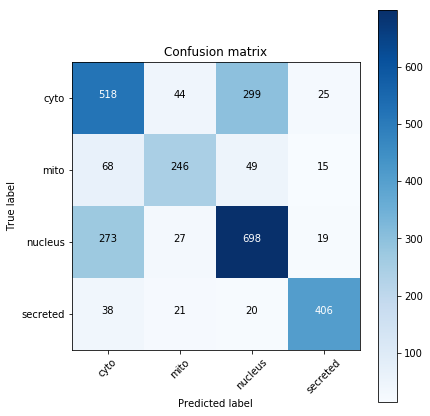
\includegraphics[width=8cm]{confusion}
\centering
\end{figure}

\begin{figure}[!h]
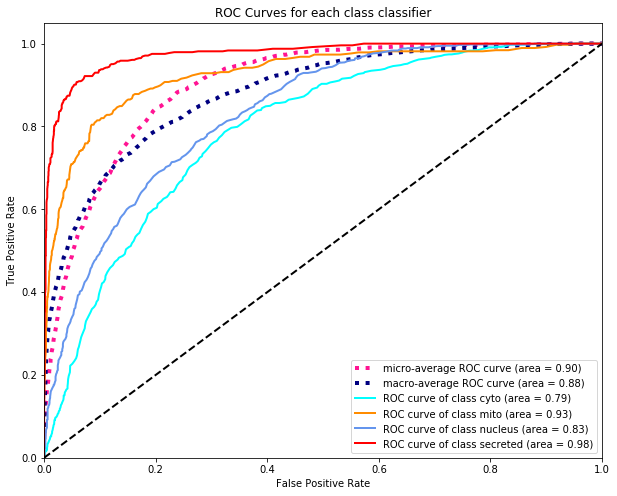
\includegraphics[width=8cm]{roc_curve}
\centering
\end{figure}

\subsection{Error Analysis}

In inspecting our best performing model, Random Forests, more closely, it is clear that the errors in the model were not distributed evenly across categories.
Instead it appears that the greatest source error in fact come from misclassifying nuclear labels for cytosolic ones. This can be seen clearly from the confusion matrix presented in \textit{confusion matrix}. Almost $X\%$ of nuclear proteins are misclassified as cytosolic, and $Y\%$ as cytosolic as nuclear.

This misclassification is made all the more evident by looking at the Returning Order Characteristic (ROC) curves, where all the classifiers are plotted together. 
From these graphs, it is immediately clear that the best classifier is the secreted class, with the area under curve (AUC) of 0.98, followed by the mitochondrial class of 0.93. The worst performer is the cytosolic class (0.79) followed by the nuclear class (0.83).

There are a number of reasons why it is conceivable that these particular protein classifiers (cytosolic and nuclear) should perform worse than the other two categories (secreted and mitochondrial). 
For one thing, there are a number of proteins that frequently move between the nucleus and the cytoplasm, meaning that they may posses both \textit{Nuclear Export Signals} and \textit{Nuclear Localization Signals}. 
This mixup of very distinct features (in the form of target peptides) would likely lead the classifiers to struggle to distinguish the correct class in ambiguous cases.

Furthermore, it is likely that mitochondrial proteins and secreted proteins may have important properties that are unrelated to target peptides but still show up in our choice of features. For instance, since secreted proteins need to cross the cell membrane, it is possible features such as very large size or certain peptide make up, might make this action difficult. There may exist alternative restrictions on mitochondrial proteins, that need to be adapted to help in respiration, which might also restrict the protein's structure.

At any rate it is clear from the ROC curves in particular that secretion is particularly well detected, with \textit{comment about false positives etc}, nuclear and cytoplasmic classes are easier to confuse. An analysis of the exact features that could be responsible for this are presented in the next section.


% As mentioned previously, peptides destined for a certain subcellular location often have sequences of peptides encoding this. It is likely these are strong features in this sequence analysis, and will be examined in the netx Furthermore, it is likely that peptides operating in a certain part of the cell might have specific features, related to it specific function

% The strength of the secreted and mitochondrial classes i two classes as classifiers is at least partly down to the very specific nature of proteins these locations. For a protein to be secreted, there is a requirement that it is able to be transported across the cell membrane, and this puts some restrictions on the form the protein can take. \textbf{what restriction}. Similarly the mitochondrial proteins are highly likely to be used in respiration in some respect and so are likely again to have features that indicate this. 
% However, there are many proteins that are frequently transported between the nucleus and the cytosol, meaning that it can be hard to distinguish these proteins from features.
% A more specific look at the features, and what they can be used to discern, is examined in the following section.
\begin{figure}[!h]
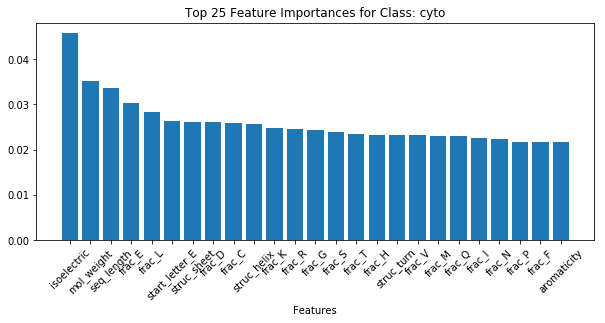
\includegraphics[width=8cm]{cyto_import}
\centering
% \end{figure}\begin{figure}[h]
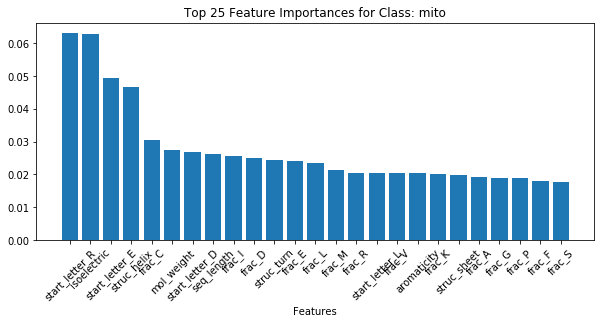
\includegraphics[width=8cm]{mito_import}
\centering
% \end{figure}\begin{figure}[h]
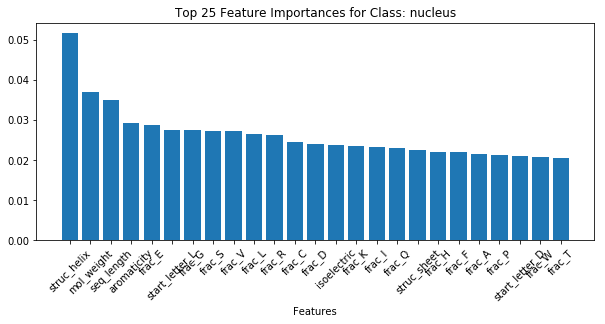
\includegraphics[width=8cm]{nucleus_import}
\centering
% \end{figure}\begin{figure}[h]
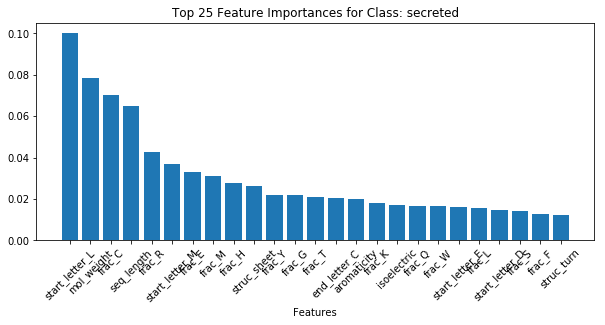
\includegraphics[width=8cm]{secreted_import}
\centering
\end{figure}

\subsection{Features Analysis}

Perhaps more interesting than the comparison of the two different models is the close comparison of the features that have had a significant impact on the model.
Thankfully, our One-Vs-Rest Random Forest Model has an in built way of examining the features, via the feature importances.
These are displayed in figure \text{ref importances}.

The first thing to notice is the relative scales of the four graphs, in comparison to one another. The secreted classifier has a much stronger set of "significant" features, than all the other classes. In the case of comparison to nucleus and cytoplasmic classes, secreted's top feature is over twice the importance of the latter classes highest feature. Furthermore its top 4 features features all have higher importances than the highest single feature for these classes.  This indicates that there are distinct "killer features" for this class, and it appears they are highly tied to the fraction of Leucines and Cysteines at the start of the sequence, and the molecular weight and sequence length. \textbf{investigate data?}

Next to notice is that, as mentioned in the initial background, mitochondrial proteins also have importances supporting the target peptides alluded to. 
\textit{Mitochondrial targeting signals} sometimes consist of alternating positively charged and hydrophobic amino acids forming a helix, so unsurprisingly our strongest features include features noting isoelectricity, structural helices, and the presence of positively charged Arginine at the start of the sequences.

When it comes to nuclear and cytosolic proteins, it's worth noting that the second and third best importance features are shared - indicating the difficulty these  classes might have in distinguishing themselves.  Furthermore these features - molecular weight and sequence length - are broad macroscopic features that do not really indicate a particular target sequence, and also show why it might be hard to classify these proteins. Even the "strongest feature" for these two classes is a macroscropic feature - isoelectric point, and percentage of "common helix" amino acids, indicating our set of features haven't been able to pick up the nuclear target peptides.

Finally it is worth noting that none of the most important features correspond to peptides at the end of the sequence.  This is fairly good evidence that something important happens at the N-terminus of a protein, and  supports background theory that this is where target peptides are often found.


\subsection{Further Improvements}

Although this model performed well in distinguishing the secreted and mitochondrial proteins there are a number of additional features that may particularly improve future implementations of this model. 

First, some measure of hydrophobicity would be a valuable additional feature. This wasn't added due to the lack of there being an available scale in the BioPython module, but it is likely this addition would help to pick up the hydrophobicity of of elements found in \textit{either NLS or NES sections of the sequence}, helping to distiguish nuclear and cytoplasmic proteins.

Furthermore it should be worth exploring and searching for specific target patterns within the model. I attempted to search for these by creating a feature for all possible "bigrams" and "trigrams" of residues, and looking at importances, but the high dimensionality made learning difficult. Instead, if one had specific examples of known target peptides this feature would likely greatly help classification, without adding too much to computational complexity.

Finally it may be worth trying gradient boosting algorithms or neural networks. Gradient boostin algorithms such as XGBoost \textit{Explain why gradient boosting maybe better 2 lines}. Neural networks also have significant performance, but mainly on high data sets. Given the relatively small dataset (only a few \textit{thousand points}), neural methods may not be suited to this particular small task.

\section{Conclusions}



%     - Results of accuracy
%     - Confusion matrix
%     - ablation study
%     - results compared to xgboost


% Judging by the results of the confusion matrix and ROC Curves, it is clear the model greatly succeed in labelling some categories while struggling with others. In particular, it was able to classify secreted and mitochondrial proteins with much more success than nuclear and cytosolic proteins. \textit{X\%} of secreted proteins were classified correctly, along with \textit{X\%} of mitochondrial proteins. \textit{Precision and recall}. 

% These locations are it is likely that these locations 

%  This is likely both  down the similarity of the nuclear and cytosolic proteins, and the lack of an appropriate discriminating feature to distinguish their similarty.


  


% \subsection{Classifier Analysis}

% \subsection{Model Evaluation Analysis}




\newpage
yip
\newpage

Obtained data from X files, and mixed, shuffle and split into a train and validation split. Since the proteins are all non homologues, no need to arrange by family and could split anyway. 

Then took these files and processed them into feature vectors, using the bipython module. These extracted, x features from the sequence. 

Then trained a random forest classifier with X trees, and also tested a XGBboost classifier.

Cross validated grid search done to find best parameters for trees
Ablation study used to investigate salient features.

Trained a random forest with X trees. 

What did you do?
    - extract features
    - train -test split - homologies
    - cross validate
    - compared with a model (gradient boosting?)
    - ablation study



    - Results of accuracy
    - Confusion matrix
    - ablation study
    - results compared to xgboost
\section{Discussion}
   - Examine the features
   - Examine the ablation study
   - Examine comparison to XGBoost
   - Compare with existing literature and approaches



\section{Further Work}
    - suggestions: more data? better features/

\section{Conclusion}

\section{Theoretical Background}

What about ???
















\newpage
end of paper
\newpage

Text Text Text Text Text Text  Text Text Text Text Text Text Text
Text Text  Text Text Text Text Text Text. Figure~\ref{fig:01}
shows that the above method  Text Text Text Text  Text Text Text
Text Text Text  Text Text.  \citep{Bag01} wants to know about
{\ldots}{\ldots} text follows.
\begin{equation}
\sum \text{\it x}+ \text{\it y} =\text{\it Z}\label{eq:01}\vspace*{-10pt}
\end{equation}

%\enlargethispage{12pt}

\section{Approach}

Equation~(\ref{eq:01}) Text Text Text Text Text Text  Text Text
Text Text Text Text Text Text Text Text Text Text Text Text Text.
Figure~2\vphantom{\ref{fig:02}} shows that the above method  Text
Text Text Text  Text Text Text Text Text Text  Text Text.
\citealp{Boffelli03} might want to know about text text text text
.....


\begin{methods}
\section{Methods}

Text Text Text Text Text Text  Text Text Text Text Text Text Text
Text Text  Text Text Text Text Text Text.
Figure~2\vphantom{\ref{fig:02}} shows that the above method  Text
Text Text Text  Text Text Text Text Text Text  Text Text.
\citealp{Boffelli03} might want to know about  text text text text
Text Text Text Text Text Text Text Text Text Text Text Text Text
Text Text  Text Text Text Text Text Text.
Figure~2\vphantom{\ref{fig:02}} shows that the above method  Text
Text Text Text Text Text Text Text Text Text  Text Text.
\citealp{Boffelli03} might want to know about text text text text
Text Text Text Text Text Text  Text Text Text Text Text Text Text
Text Text Text Text Text Text Text Text.
Figure~2\vphantom{\ref{fig:02}} shows that the above method  Text
Text Text Text Text Text Text Text Text Text  Text Text.
\citealp{Boffelli03} might want to know about text text text
text\vspace*{1pt}

\begin{itemize}
\item for bulleted list, use itemize
\item for bulleted list, use itemize
\item for bulleted list, use itemize\vspace*{1pt}
\end{itemize}

Text Text Text Text Text Text  Text Text Text Text Text Text Text
Text Text  Text Text Text Text Text Text.
Figure~2\vphantom{\ref{fig:02}} shows that the above method  Text
Text Text Text  Text Text Text Text Text Text  Text Text.
\citealp{Boffelli03} might want to know about  text text text text
Text Text Text Text Text Text Text Text Text Text Text Text Text
Text Text Text Text Text Text Text Text.
Figure~2\vphantom{\ref{fig:02}} shows that the above method  Text
Text Text Text Text Text Text Text Text Text  Text Text.
\citealp{Boffelli03} might want to know about text text text text
Text Text Text Text Text Text  Text Text Text Text Text Text Text
Text Text Text Text Text Text Text Text.
Figure~2\vphantom{\ref{fig:02}} shows that the above method  Text
Text Text Text Text Text Text Text Text Text  Text Text.
\citealp{Boffelli03} might want to know about text text text text
Text Text Text Text Text Text  Text Text Text Text Text Text Text
Text Text Text Text Text Text Text Text.
Figure~2\vphantom{\ref{fig:02}} shows that the above method Text
Text Text Text Text Text Text Text Text Text Text Text.
\citealp{Boffelli03} might want to know about text text text text
Text Text Text Text Text Text  Text Text Text Text Text Text Text
Text Text Text Text Text Text Text Text.

Text Text Text Text Text Text  Text Text Text Text Text Text Text
Text Text  Text Text Text Text Text Text\vadjust{\newpage}.
Figure~2\vphantom{\ref{fig:02}} shows that the above method  Text
Text Text Text  Text Text Text Text Text Text  Text Text.
\citealp{Boffelli03} might want to know about text text text text
Text Text Text Text Text Text Text Text Text Text Text Text Text
Text Text Text Text Text Text Text Text.
Figure~2\vphantom{\ref{fig:02}} shows that the above method  Text
Text Text Text Text Text Text Text Text Text  Text Text.
\citealp{Boffelli03} might want to know about text text text text
Text Text Text Text Text Text  Text Text Text Text Text Text Text
Text Text Text Text Text Text Text Text.
Figure~2\vphantom{\ref{fig:02}} shows that the above method  Text
Text Text Text Text Text Text Text Text Text  Text Text.
\citealp{Boffelli03} might want to know about text text text text
Text Text Text Text Text Text  Text Text Text Text Text Text Text
Text Text Text Text Text Text Text Text.
Figure~2\vphantom{\ref{fig:02}} shows that the above method Text
Text Text Text Text Text Text Text Text Text Text Text.
\citealp{Boffelli03} might want to know about text text text text
Text Text Text Text Text Text  Text Text Text Text Text Text Text
Text Text Text Text Text Text Text Text.


Text Text Text Text Text Text  Text Text Text Text Text Text Text
Text Text  Text Text Text Text Text Text.
Figure~2\vphantom{\ref{fig:02}} shows that the above method  Text
Text Text Text  Text Text Text Text Text Text  Text Text.
\citealp{Boffelli03} might want to know about  text text text text
Text Text Text Text Text Text  Text Text Text Text Text Text Text
Text Text  Text Text Text Text Text Text.
Figure~2\vphantom{\ref{fig:02}} shows that the above method  Text
Text Text Text  Text Text Text Text Text Text  Text Text.
\citealp{Boffelli03} might want to know about  text text text text
Text Text Text Text Text Text Text Text Text Text Text Text Text
Text Text  Text Text Text Text Text Text.
Figure~2\vphantom{\ref{fig:02}} shows that the above method  Text
Text Text Text  Text Text Text Text Text Text  Text Text.
\citealp{Boffelli03} might want to know about  text text text text



Text Text Text Text Text Text  Text Text Text Text Text Text Text
Text Text  Text Text Text Text Text Text.
Figure~2\vphantom{\ref{fig:02}} shows that the above method  Text
Text Text Text  Text Text Text Text Text Text  Text Text.
\citealp{Boffelli03} might want to know about  text text text text
Text Text Text Text Text Text  Text Text Text Text Text Text Text
Text Text  Text Text Text Text Text Text.
Figure~2\vphantom{\ref{fig:02}} shows that the above method  Text
Text Text Text  Text Text Text Text Text Text  Text Text.
\citealp{Boffelli03} might want to know about  text text text text
Text Text Text Text Text Text Text Text Text Text Text Text Text
Text Text  Text Text Text Text Text Text.

\subsection{This is subheading}

Text Text Text Text Text Text  Text Text Text Text Text Text Text
Text Text  Text Text Text Text Text Text.
Figure~2\vphantom{\ref{fig:02}} shows that the above method  Text
Text Text Text  Text Text Text Text Text Text  Text Text.
\citealp{Boffelli03} might want to know about  text text text text
Text Text Text Text Text Text  Text Text Text Text Text Text Text
Text Text  Text Text Text Text Text Text.
Figure~2\vphantom{\ref{fig:02}} shows that the above method  Text
Text Text Text Text Text Text Text Text Text  Text Text.
\citealp{Boffelli03} might want to know about  text text text text
Text Text Text Text Text Text Text Text Text Text Text Text Text
Text Text  Text Text Text Text Text Text.
Figure~2\vphantom{\ref{fig:02}} shows that the above method  Text
Text Text Text Text Text Text Text Text Text  Text Text.
\citealp{Boffelli03} might want to know about  text text text
text. Text Text Text Text Text Text  Text Text Text Text Text Text
Text Text Text  Text Text Text Text Text Text.
Figure~2\vphantom{\ref{fig:02}} shows that the above method  Text
Text Text Text Text Text Text Text Text Text  Text Text.
\citealp{Boffelli03} might want to know about  text text text text
Text Text Text Text Text Text Text Text Text Text Text Text Text
Text Text  Text Text Text Text Text Text.
Figure~2\vphantom{\ref{fig:02}} shows that the above method  Text
Text Text Text Text Text Text Text Text Text  Text Text.
\citealp{Boffelli03} might want to know about  text text text text
Text Text Text Text Text Text  Text Text Text Text Text Text Text
Text Text  Text Text Text Text Text Text.
Figure~2\vphantom{\ref{fig:02}} shows that the above method  Text
Text Text Text Text Text Text Text Text Text  Text Text.
\citealp{Boffelli03} might want to know about  text text text text
Text Text Text Text Text Text Text Text Text Text Text Text Text
Text Text  Text Text Text Text Text Text.
Figure~2\vphantom{\ref{fig:02}} shows that the above method  Text
Text Text Text Text Text Text Text Text Text  Text Text.
\citealp{Boffelli03} might want to know about  text text text text
Text Text Text Text Text Text  Text Text Text Text Text Text Text
Text Text  Text Text Text Text Text Text.


\subsubsection{This is subsubheading}

Text Text Text Text Text Text  Text Text Text Text Text Text Text
Text Text  Text Text Text Text Text Text.
Figure~2\vphantom{\ref{fig:02}} shows that the above method  Text
Text Text Text  Text Text Text Text Text Text  Text Text.
\citealp{Boffelli03} might want to know about  text text text text
Text Text Text Text Text Text  Text Text Text Text Text Text Text
Text Text  Text Text Text Text Text Text.
Figure~2\vphantom{\ref{fig:02}} shows that the above method  Text
Text Text Text  Text Text Text Text Text Text  Text Text.
\citealp{Boffelli03} might want to know about  text text text text
Text Text Text Text Text Text Text Text Text Text Text Text Text
Text Text  Text Text Text Text Text Text.
Figure~2\vphantom{\ref{fig:02}} shows that the above method  Text
Text Text Text  Text Text Text Text Text Text  Text Text.
\citealp{Boffelli03} might want to know about  text text text text



Text Text Text Text Text Text  Text Text Text Text Text Text Text
Text Text  Text Text Text Text Text Text.
Figure~2\vphantom{\ref{fig:02}} shows that the above method  Text
Text Text Text  Text Text Text Text Text Text  Text Text.
\citealp{Boffelli03} might want to know about  text text text text
Text Text Text Text Text Text  Text Text Text Text Text Text Text
Text Text  Text Text Text Text Text Text.
Figure~2\vphantom{\ref{fig:02}} shows that the above method  Text
Text Text Text  Text Text Text Text Text Text  Text Text.
\citealp{Boffelli03} might want to know about  text text text text
Text Text Text Text Text Text Text Text Text Text Text Text Text
Text Text  Text Text Text Text Text Text.
Figure~2\vphantom{\ref{fig:02}} shows that the above method  Text
Text Text Text  Text Text Text Text Text Text  Text Text.
\citealp{Boffelli03} might want to know about  text text\break
text text


Text Text Text Text Text Text  Text Text Text Text Text Text Text
Text Text  Text Text Text Text Text Text.
Figure~2\vphantom{\ref{fig:02}} shows that the above method  Text
Text Text Text  Text Text Text Text Text Text  Text Text.
\citealp{Boffelli03} might want to know about  text text text text
Text Text Text Text Text Text  Text Text Text Text Text Text Text
Text Text  Text Text Text Text Text Text.
Figure~2\vphantom{\ref{fig:02}} shows that the above method  Text
Text Text Text  Text Text Text Text Text Text  Text Text.
\citealp{Boffelli03} might want to know about  text text text text
Text Text Text Text Text Text Text Text Text Text Text Text Text
Text Text  Text Text Text Text Text Text.
Figure~2\vphantom{\ref{fig:02}} shows that the above method  Text
Text Text Text  Text Text Text Text Text Text  Text Text.
\citealp{Boffelli03} might want to know about  text text text
textText Text Text Text Text Text  Text Text Text Text Text Text
Text Text Text  Text Text Text Text Text Text.
Figure~2\vphantom{\ref{fig:02}} shows that the above method  Text
Text Text Text  Text Text Text Text Text Text  Text Text.
\citealp{Boffelli03} might want to know about  text text text text
Text Text Text Text Text Text Text Text Text Text Text Text Text
Text Text  Text Text Text Text Text Text.
Figure~2\vphantom{\ref{fig:02}} shows that the above method  Text
Text Text Text  Text Text Text Text Text Text  Text Text.
\citealp{Boffelli03} might want to know about  text text text text
Text Text Text Text Text Text  Text Text Text Text Text Text Text
Text Text  Text Text Text Text Text Text.
Figure~2\vphantom{\ref{fig:02}} shows that the above method  Text
Text Text Text  Text Text Text Text Text Text  Text Text.
\citealp{Boffelli03} might want to know about  text text text text
Text Text Text Text Text Text Text Text Text Text Text Text Text
Text Text  Text Text Text Text Text Text.
Figure~2\vphantom{\ref{fig:02}} shows that the above method  Text
Text Text Text  Text Text Text Text Text Text  Text Text.
\citealp{Boffelli03} might want to know about  text text text text
Text Text Text Text Text Text  Text Text Text Text Text Text Text
Text Text  Text Text Text Text Text Text.

\enlargethispage{6pt}


Text Text Text Text Text Text  Text Text Text Text Text Text Text
Text Text  Text Text Text Text Text Text.
Figure~2\vphantom{\ref{fig:02}} shows that the above method  Text
Text Text Text  Text Text Text Text Text Text  Text Text.
\citealp{Boffelli03} might want to know about  text text text text
Text Text Text Text Text Text  Text Text Text Text Text Text Text
Text Text  Text Text Text Text Text Text.
Figure~2\vphantom{\ref{fig:02}} shows that the above method  Text
Text Text Text  Text Text Text Text Text Text  Text Text.
\citealp{Boffelli03} might want to know about  text text text text
Text Text Text Text Text Text Text Text Text Text Text Text Text
Text Text  Text Text Text Text Text Text.
Figure~2\vphantom{\ref{fig:02}} shows that the above method  Text
Text Text Text  Text Text Text Text Text Text  Text Text.
\citealp{Boffelli03} might want to know about  text text text text



Text Text Text Text Text Text  Text Text Text Text Text Text Text
Text Text  Text Text Text Text Text Text.
Figure~2\vphantom{\ref{fig:02}} shows that the above method  Text
Text Text Text  Text Text Text Text Text Text  Text Text.
\citealp{Boffelli03} might want to know about  text text text text
Text Text Text Text Text Text  Text Text Text Text Text Text Text
Text Text  Text Text Text Text Text Text.
Figure~2\vphantom{\ref{fig:02}} shows that the above method  Text
Text Text Text  Text Text Text Text Text Text  Text Text.
\citealp{Boffelli03} might want to know about  text text text text
Text Text Text Text Text Text Text Text Text Text Text Text Text
Text Text  Text Text Text Text Text Text.
Figure~2\vphantom{\ref{fig:02}} shows that the above method  Text
Text Text Text  Text Text Text Text Text Text  Text Text.
\citealp{Boffelli03} might want to know about  text text text text


Text Text Text Text Text Text  Text Text Text Text Text Text Text
Text Text  Text Text Text Text Text Text.
Figure~2\vphantom{\ref{fig:02}} shows that the above method  Text
Text Text Text  Text Text Text Text Text Text  Text Text.
\citealp{Boffelli03} might want to know about  text text text text
Text Text Text Text Text Text  Text Text Text Text Text Text Text
Text Text  Text Text Text Text Text Text.
Figure~2\vphantom{\ref{fig:02}} shows that the above method  Text
Text Text Text  Text Text Text Text Text Text  Text Text.
\citealp{Boffelli03} might want to know about  text text text text
Text Text Text Text Text Text Text Text Text Text Text Text Text
Text Text  Text Text Text Text Text Text.
Figure~2\vphantom{\ref{fig:02}} shows that the above method  Text
Text Text Text  Text Text Text Text Text Text  Text Text.
\citealp{Boffelli03} might want to know about  text text text text

Text Text Text Text Text Text  Text Text Text Text Text Text Text
Text Text  Text Text Text Text Text Text.
Figure~2\vphantom{\ref{fig:02}} shows that the above method  Text
Text Text Text  Text Text Text Text Text Text  Text Text.
\citealp{Boffelli03} might want to know about  text text text text
Text Text Text Text Text Text  Text Text Text Text Text Text Text
Text Text  Text Text Text Text Text Text.
Figure~2\vphantom{\ref{fig:02}} shows that the above method  Text
Text Text Text  Text Text Text Text Text Text  Text Text.
\citealp{Boffelli03} might want to know about  text text text text
Text Text Text Text Text Text Text Text Text Text Text Text Text
Text Text  Text Text Text Text Text Text.
Figure~2\vphantom{\ref{fig:02}} shows that the above method  Text
Text Text Text  Text Text Text Text Text Text  Text Text.
\citealp{Boffelli03} might want to know about  text text text text
Text Text Text Text Text Text  Text Text Text Text Text Text Text
Text Text  Text Text Text Text Text Text.
Figure~2\vphantom{\ref{fig:02}} shows that the above method  Text
Text Text Text  Text Text Text Text Text Text  Text Text.
\citealp{Boffelli03} might want to know about  text text text text
Text Text Text Text Text Text Text Text Text Text Text Text Text
Text Text  Text Text Text Text Text Text.


Text Text Text Text Text Text  Text Text Text Text Text Text Text
Text Text  Text Text Text Text Text Text.
Figure~2\vphantom{\ref{fig:02}} shows that the above method  Text
Text Text Text  Text Text Text Text Text Text  Text Text.
\citealp{Boffelli03} might want to know about  text text text text
Text Text Text Text Text Text  Text Text Text Text Text Text Text
Text Text  Text Text Text Text Text Text.
Figure~2\vphantom{\ref{fig:02}} shows that the above method  Text
Text Text Text  Text Text Text Text Text Text  Text Text.
\citealp{Boffelli03} might want to know about  text text text text
Text Text Text Text Text Text Text Text Text Text Text Text Text
Text Text  Text Text Text Text Text Text.
Figure~2\vphantom{\ref{fig:02}} shows that the above method  Text
Text Text Text  Text Text Text Text Text Text  Text Text.
\citealp{Boffelli03} might want to know about  text text text text

\begin{table}[!t]
\processtable{This is table caption\label{Tab:01}} {\begin{tabular}{@{}llll@{}}\toprule head1 &
head2 & head3 & head4\\\midrule
row1 & row1 & row1 & row1\\
row2 & row2 & row2 & row2\\
row3 & row3 & row3 & row3\\
row4 & row4 & row4 & row4\\\botrule
\end{tabular}}{This is a footnote}
\end{table}

\end{methods}

\begin{figure}[!tpb]%figure1
\fboxsep=0pt\colorbox{gray}{\begin{minipage}[t]{235pt} \vbox to 100pt{\vfill\hbox to
235pt{\hfill\fontsize{24pt}{24pt}\selectfont FPO\hfill}\vfill}
\end{minipage}}
%\centerline{\includegraphics{fig01.eps}}
\caption{Caption, caption.}\label{fig:01}
\end{figure}

%\begin{figure}[!tpb]%figure2
%%\centerline{\includegraphics{fig02.eps}}
%\caption{Caption, caption.}\label{fig:02}
%\end{figure}

Text Text Text Text Text Text  Text Text Text Text Text Text Text
Text Text  Text Text Text Text Text Text.
Figure~2\vphantom{\ref{fig:02}} shows that the above method  Text
Text Text Text  Text Text Text Text Text Text  Text Text.
\citealp{Boffelli03} might want to know about  text text text text
Text Text Text Text Text Text  Text Text Text Text Text Text Text
Text Text  Text Text Text Text Text Text.
Figure~2\vphantom{\ref{fig:02}} shows that the above method  Text
Text Text Text  Text Text Text Text Text Text  Text Text.
\citealp{Boffelli03} might want to know about  text text text text
Text Text Text Text Text Text Text Text Text Text Text Text Text
Text Text  Text Text Text Text Text Text.
Figure~2\vphantom{\ref{fig:02}} shows that the above method  Text
Text Text Text  Text Text Text Text Text Text  Text Text.
\citealp{Boffelli03} might want to know about  text text text text


\subsection{Test1}

Text Text Text Text Text Text  Text Text Text Text Text Text Text
Text Text  Text Text Text Text Text Text.
Figure~2\vphantom{\ref{fig:02}} shows that the above method  Text
Text Text Text  Text Text Text Text Text Text  Text Text.
\citealp{Boffelli03} might want to know about  text text text text
Text Text Text Text Text Text  Text Text Text Text Text Text Text
Text Text  Text Text Text Text Text Text.
Figure~2\vphantom{\ref{fig:02}} shows that the above method  Text
Text Text Text  Text Text Text Text Text Text  Text Text.
\citealp{Boffelli03} might want to know about  text text text text
Text Text Text Text Text Text Text Text Text Text Text Text Text
Text Text  Text Text Text Text Text Text.
Figure~2\vphantom{\ref{fig:02}} shows that the above method  Text
Text Text Text  Text Text Text Text Text Text  Text Text.
\citealp{Boffelli03} might want to know about  text text text text





\section{Discussion}

Text Text Text Text Text Text  Text Text Text Text Text Text Text
Text Text  Text Text Text Text Text Text.
Figure~2\vphantom{\ref{fig:02}} shows that the above method  Text
Text Text Text  Text Text Text Text Text Text  Text Text.
\citealp{Boffelli03} might want to know about  text text text text
Text Text Text Text Text Text  Text Text Text Text Text Text Text
Text Text  Text Text Text Text Text Text.
Figure~2\vphantom{\ref{fig:02}} shows that the above method  Text
Text Text Text  Text Text Text Text Text Text  Text Text.
\citealp{Boffelli03} might want to know about  text text text text
Text Text Text Text Text Text Text Text Text Text.




Table~\ref{Tab:01} shows that Text Text Text Text Text  Text Text
Text Text Text Text. Figure~2\vphantom{\ref{fig:02}} shows that
the above method Text Text. Text Text Text  Text Text Text Text
Text Text. Figure~2\vphantom{\ref{fig:02}} shows that the above
method Text Text. Text Text Text  Text Text Text Text Text Text.
Figure~2\vphantom{\ref{fig:02}} shows that the above method Text
Text.









%%%%%%%%%%%%%%%%%%%%%%%%%%%%%%%%%%%%%%%%%%%%%%%%%%%%%%%%%%%%%%%%%%%%%%%%%%%%%%%%%%%%%
%
%     please remove the " % " symbol from \centerline{\includegraphics{fig01.eps}}
%     as it may ignore the figures.
%
%%%%%%%%%%%%%%%%%%%%%%%%%%%%%%%%%%%%%%%%%%%%%%%%%%%%%%%%%%%%%%%%%%%%%%%%%%%%%%%%%%%%%%






\section{Conclusion}

(Table~\ref{Tab:01}) Text Text Text Text Text Text  Text Text Text
Text Text Text Text Text Text  Text Text Text Text Text Text.
Figure~2\vphantom{\ref{fig:02}} shows that the above method  Text
Text Text Text  Text Text Text Text Text Text  Text Text.
\citealp{Boffelli03} might want to know about  text text text text
Text Text Text Text Text Text  Text Text Text Text Text Text Text
Text Text  Text Text Text Text Text Text.
Figure~2\vphantom{\ref{fig:02}} shows that the above method  Text
Text Text Text  Text Text Text Text Text Text  Text Text.
\citealp{Boffelli03} might want to know about  text text text text
Text Text Text Text Text Text Text Text Text Text Text Text Text
Text Text  Text Text Text Text Text Text.
Figure~2\vphantom{\ref{fig:02}} shows that the above method  Text
Text Text Text  Text Text Text Text Text Text  Text Text.



Text Text Text Text Text Text  Text Text Text Text Text Text Text
Text Text  Text Text Text Text Text Text.
Figure~2\vphantom{\ref{fig:02}} shows that the above method  Text
Text Text Text  Text Text Text Text Text Text  Text Text.
\citealp{Boffelli03} might want to know about  text text text text

\begin{enumerate}
\item this is item, use enumerate
\item this is item, use enumerate
\item this is item, use enumerate
\end{enumerate}

Text Text Text Text Text Text Text Text Text Text Text Text Text
Text Text Text Text Text Text Text Text.
Figure~2\vphantom{\ref{fig:02}} shows\vadjust{\pagebreak} that the
above method  Text Text Text Text Text Text Text Text Text Text
Text Text.  \citealp{Boffelli03} might want to know about text
text text text Text Text Text Text Text Text  Text Text Text Text
Text Text Text Text Text Text Text Text Text Text Text.
Figure~2\vphantom{\ref{fig:02}} shows that the above method  Text
Text Text Text Text Text Text Text Text Text  Text Text.
\citealp{Boffelli03} might want to know about text text text text
Text Text Text Text Text Text  Text Text Text Text Text Text Text
Text Text Text Text Text Text Text\break Text.


Text Text Text Text Text Text  Text Text Text Text Text Text Text
Text Text  Text Text Text Text Text Text.
Figure~2\vphantom{\ref{fig:02}} shows that the above method  Text
Text Text Text\vspace*{-10pt}


\section*{Acknowledgements}

Text Text Text Text Text Text  Text Text.  \citealp{Boffelli03} might want to know about  text
text text text\vspace*{-12pt}

\section*{Funding}

This work has been supported by the... Text Text  Text Text.\vspace*{-12pt}

%\bibliographystyle{natbib}
%\bibliographystyle{achemnat}
%\bibliographystyle{plainnat}
%\bibliographystyle{abbrv}
%\bibliographystyle{bioinformatics}
%
%\bibliographystyle{plain}
%
%\bibliography{Document}


\begin{thebibliography}{}

\bibitem[Bofelli {\it et~al}., 2000]{Boffelli03}
Bofelli,F., Name2, Name3 (2003) Article title, {\it Journal Name}, {\bf 199}, 133-154.

\bibitem[Bag {\it et~al}., 2001]{Bag01}
Bag,M., Name2, Name3 (2001) Article title, {\it Journal Name}, {\bf 99}, 33-54.

\bibitem[Yoo \textit{et~al}., 2003]{Yoo03}
Yoo,M.S. \textit{et~al}. (2003) Oxidative stress regulated genes
in nigral dopaminergic neurnol cell: correlation with the known
pathology in Parkinson's disease. \textit{Brain Res. Mol. Brain
Res.}, \textbf{110}(Suppl. 1), 76--84.

\bibitem[Lehmann, 1986]{Leh86}
Lehmann,E.L. (1986) Chapter title. \textit{Book Title}. Vol.~1, 2nd edn. Springer-Verlag, New York.

\bibitem[Crenshaw and Jones, 2003]{Cre03}
Crenshaw, B.,III, and Jones, W.B.,Jr (2003) The future of clinical
cancer management: one tumor, one chip. \textit{Bioinformatics},
doi:10.1093/bioinformatics/btn000.

\bibitem[Auhtor \textit{et~al}. (2000)]{Aut00}
Auhtor,A.B. \textit{et~al}. (2000) Chapter title. In Smith, A.C.
(ed.), \textit{Book Title}, 2nd edn. Publisher, Location, Vol. 1, pp.
???--???.

\bibitem[Bardet, 1920]{Bar20}
Bardet, G. (1920) Sur un syndrome d'obesite infantile avec
polydactylie et retinite pigmentaire (contribution a l'etude des
formes cliniques de l'obesite hypophysaire). PhD Thesis, name of
institution, Paris, France.

\end{thebibliography}
\end{document}
